
%%%%%%%%%%%%%%%%%%%%%%%%%%%%%%%%%%%%%%%%%%%%%%%%%%%%%%%%%%%%%%%%%%%%%%%
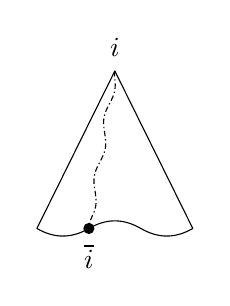
\begin{tikzpicture}[
edge from parent path=,
level distance=2cm,
level/.style={sibling distance=0.66cm/#1}
%,scale=1, every node/.style={transform shape}
]

  \tikzstyle{ref}=[circle,fill=black,inner sep=0.5mm]
  \tikzstyle{dashdot}=[dashed,dash pattern=on 2pt off 1pt on 0.5pt off 1pt]
  \tikzstyle{mysnake}=[decorate,decoration={snake,amplitude=0.4mm,segment length=0.75cm}]

  \node (c1) {}
    child { node (c2) {} }
    child { node (c3) [ref,label={below:$\overline{i}$}] {} }
    child { node (c4) {} }
    child { node (c5) {} };

  \node (c0) [minimum height=0.5cm,node distance=0.3cm,above of=c1] {$i$};

  \draw [join=round] (c1.center)
     to (c2.center) 
     to [bend right] (c3.center)
     to [bend left] (c4.center)
     to [bend right] (c5.center)
     -- cycle;

  \draw [mysnake,dashdot] (c1.center) -- (c3.center);

\end{tikzpicture}
